\section{ SM01US23 }


\subsection{Meta}

    \textbf{Title:}
    Ensemble Learning for Addressing Class Imbalance in Cardiology Appointment Scheduling and Overbooking

    \begin{table}[H]
        \centering
        \begin{tabular}{|c|c|c|c|c|c|c|c|c|}
            \hline
                \textbf{Rank} & \textbf{Grasp} & \textbf{Grade} & \textbf{Type} & \textbf{Outcome} & \textbf{Domain} & \textbf{COV19} & \textbf{CoI} & \textbf{DB} \\
            \hline
                5 & 87\% & B & A & P & A & Yes & - & Yes \\
            \hline
        \end{tabular}
        \caption{Reference's metadata}
        \label{tab:SM01US23}
    \end{table}

\subsection{Summary}
Roya Agharifar, Greg Servis, and Mohammad Khasawneh demonstrated an Ensemble Learning Prediction Model for no-show appointments in the radiology department with consideration of patient demographic data, medical records of previous appointments, and weather records. First, the authors analysed and reflected on existing studies. The medical data is represented by one year of EPIC Clarity Medical Records, and the weather records are taken from the National Centers for Environment Information, 2022. The cleaning, preparation, balancing, and analysis of medical data were performed. The prediction model consists of 3 types of algorithms bandle together by meta-model. The results yield up to 95.33\% precision. In conclusion, the obstacles, research gaps, current research gains, and further work were underlined.
    

\subsection{Notes}
    \begin{itemize}
        \item EPIC Clarity Medical Record SQL database;
        \item No-show prediction considering weather;
        \item Weather data from National Centers for Environment Information (NCEI, 2022);
        \item Has the legend of dataset structure table;
        \item RepeatedStratifiedKFold splits classes in roughly the same distribution;
    \end{itemize}


\subsection{Reading}

    \textbf{Abstract:}
    The authors analyse the missing appointments in radiology through lense of the existing literature. The new prediction model was developed and evaluated for estimating the whether a patient will atend the appointment.

    \textbf{Objectives:}
    The objective of this research is to analyse the patients behaviour of missing radiology appoinmtents and addressing the issue with prediction model.

    \textbf{Page 1:}
    The introduction of the work provides motivation for efficient no-show prediction of the healthcare services. Overbooking is a contermeasure which can be applyed if there is a high risk of missng the appointment. By overbooking in risks of no-shows the utilisation of the medical resources is going to increase.

    \textbf{Page 2:}
    Use machine learning technics to improve no-show prediction.
    
    \textbf{Page 3:}
    There are multiple factors which deretmin likelyhood of missing the appointment by patients: forgetting, socioeconomic factor, location, miscommunication. The existing studies considering patients demographic data as well as historic data of previouse appointments for input in prediction models.
    
    \textbf{Page 4:}
    In this page the authors show particular studies with the prediction models and analysis of the no-show reasons. Some works introduced that marial status, employment, employer, language, agen, and insurance are also critical factors which influance the prediction results.
    
    \textbf{Page 5:}
    There are vfew strategies to reduce effect of no-shows. First, remind patients about an appointment, overbook days when the risk of the no-show is high, increase patients aweirness by phone calls and other medium. The critaria by which the no-show is quantified and evaluated differes from study to study in addition the factors of weather are not taken into consideration for the most part.

    \textbf{Page 6:}
    The obsticles on the way of prediction model implementation is the posibility of biased decissions.
    \begin{figure}[H]
        \centering
        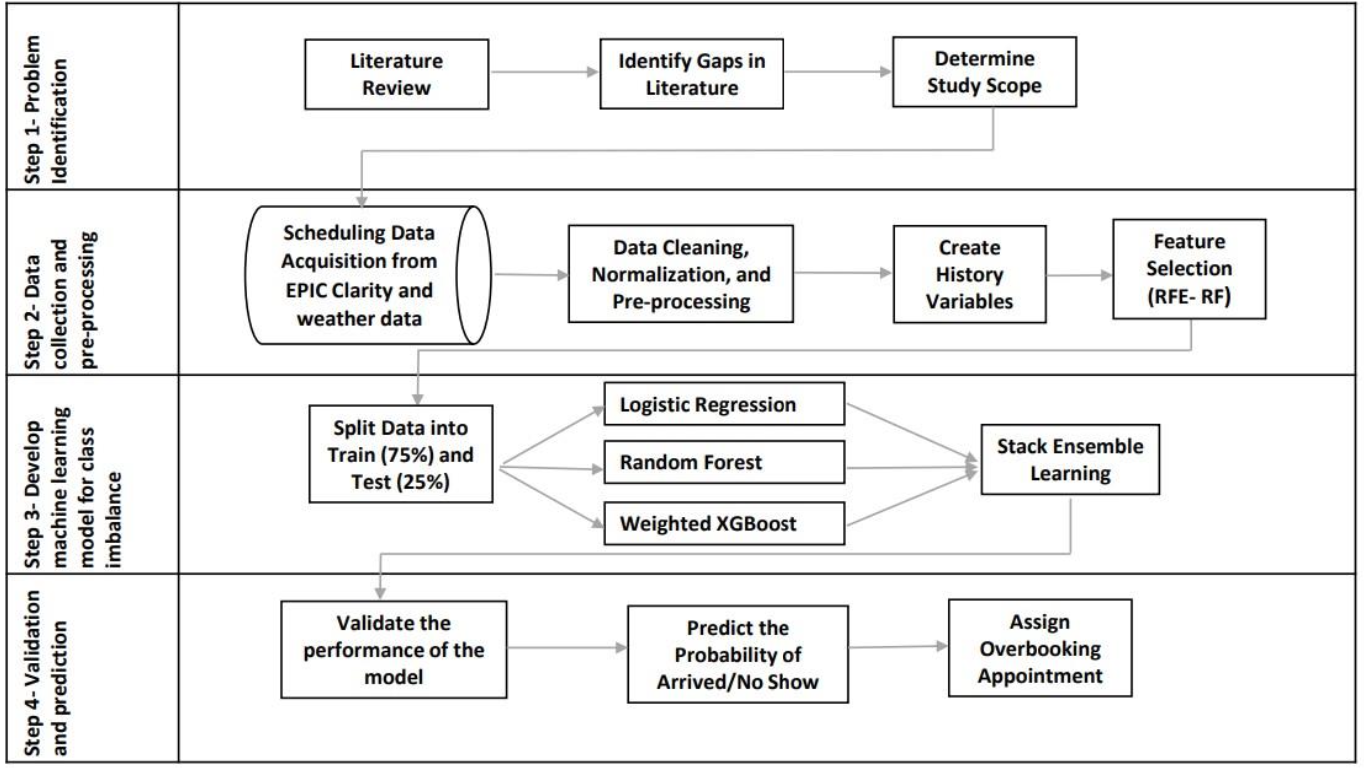
\includegraphics[width=1\textwidth]{figures/0006_SM01US23/fig1.png}
        \caption{Research methodology framework from \cite{x147}.}
        \label{fig1:0006_SM01US23}
    \end{figure}

    \textbf{Page 7:}
    The medical records and weather data were download from open source databases. In cardiology department at MSHS NYC from October 2021 to September 2022 there are almost 80,000 vists, from which 75.1\% patients arrived and the rest are no-shows.

    \textbf{Page 8:}
    The authors stated that the number of appointments influance the risk of missing the appointment (my thought is that probability theory when we have small and large numbers of visits can disrupt an interpretation of the data). Next the requred data for prediction is mined from medical and weather records and prepared.

    \textbf{Page 9:}
    The start of this page is a legend table of dataset structure. Then the open hours for appointments and general analysis of the critaria-arrival are shown.
    
    \textbf{Page 10:}
    The further the appointment is in advance the more likely that patient will cont come. In addition, older people tent to be more responsible and miss less appointments than younger people.
    
    \textbf{Page 11:}
    There is comple opposite tendencies to eldery than to young generation. Elgery people are scheduling their hospital visits far in advance, when younger people have longer time spent with physicists.
    \begin{figure}[H]
        \centering
        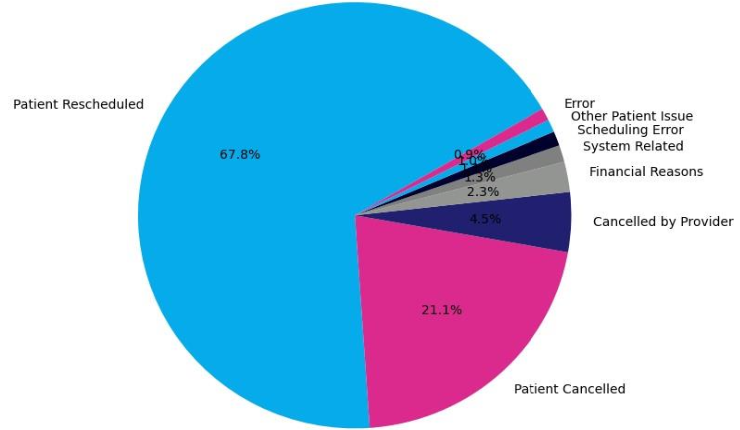
\includegraphics[width=.8\textwidth]{figures/0006_SM01US23/fig2.png}
        \caption{Research methodology framework from \cite{x147}.}
        \label{fig2:0006_SM01US23}
    \end{figure}

    \textbf{Page 12:}
    The authors explained how they addressed uneven disttribution of classes in the dataset. Then the description of the prediction model was provided, which uses bagging (multiple models on different subsets). The data was distributer training to testing in the next way: October 2021 - April 2022 (75\%) to May - September 2022 (25\%) \textit{(my consern here is that the tendencies in different seasons and even months can also different, which is not taken into account here)}

    \textbf{Page 13:}
    The data samples were also balanced in rate of no-shows to arrivals.
    \begin{figure}[H]
        \centering
        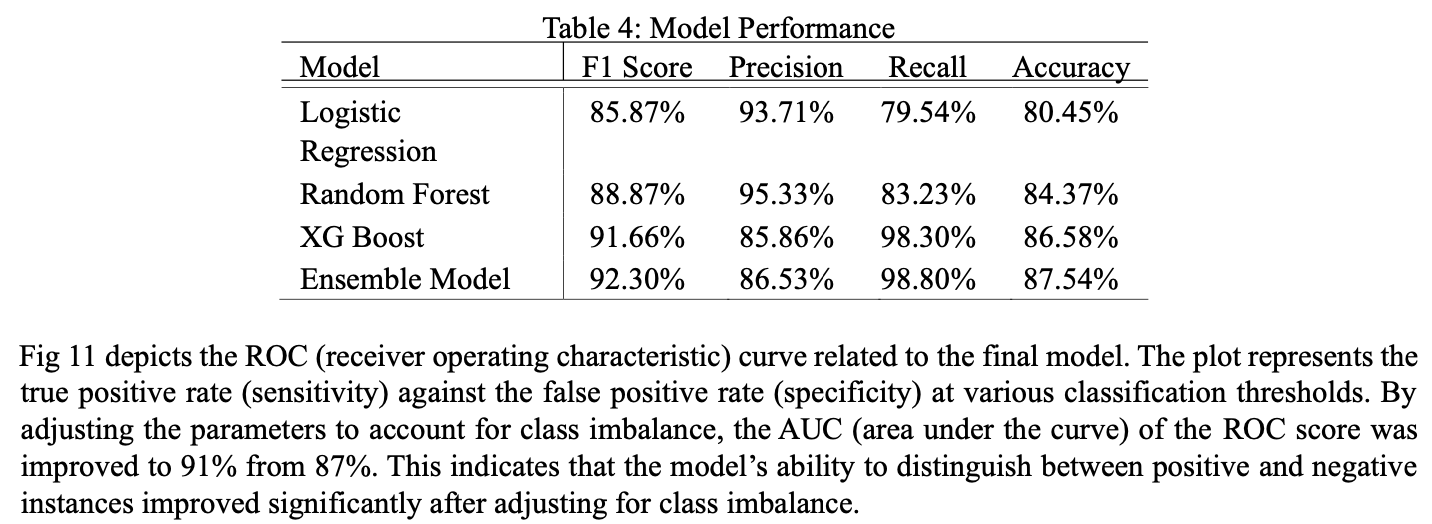
\includegraphics[width=1\textwidth]{figures/0006_SM01US23/fig4.png}
        \caption{Preformance of the prediction model from \cite{x147}.}
        \label{fig4:0006_SM01US23}
    \end{figure}
    \begin{figure}[H]
        \centering
        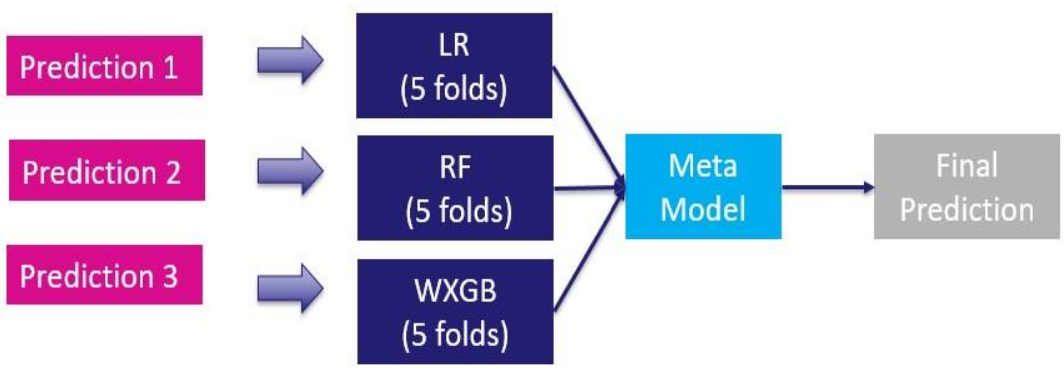
\includegraphics[width=.8\textwidth]{figures/0006_SM01US23/fig3.png}
        \caption{Architecture of the prediction model from \cite{x147}.}
        \label{fig3:0006_SM01US23}
    \end{figure}
    
    
    \textbf{Page 14:}
    The trained model shows good results and balance between precision and recall. Most of the assumtion regarding the no-shows were prooved. Some metrics like distance, pm, and maximum temperature showed no effect on the prediction outcomes, so there metrics where removed from the model.

    \textbf{Page 15:}
    The overbooking was estimated with consideration of no-show risk and patient's waiting time.
    \begin{figure}[H]
        \centering
        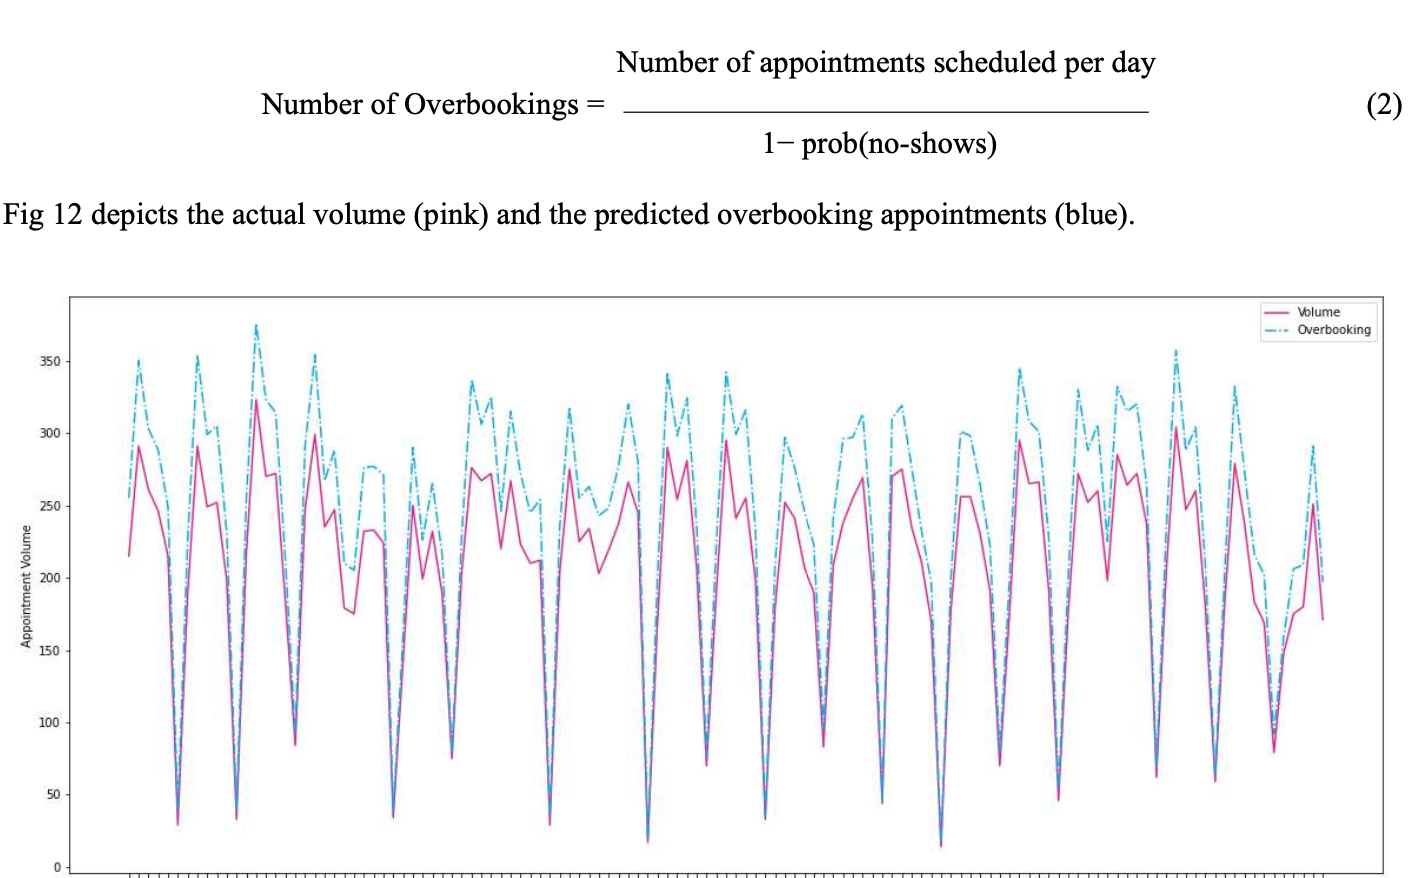
\includegraphics[width=.8\textwidth]{figures/0006_SM01US23/fig5.png}
        \caption{Overbook prediction in \cite{x147}.}
        \label{fig5:0006_SM01US23}
    \end{figure}

    \textbf{Conclusion:}
    In the conclusion, the authors hightlight the importance of the prediction of appointment no-shows, performance of the developed model, need of practical implementation, advantages of overbooking, and possibility to connect morning and afternoon appointments in the way that the model could overbook at the morning to balance afternoon bookings. Last but not least the patients income level and race could be in benefit to the prediction model.